\section{Description of the Robinhood Dataset}
The dataset records the number of Robinhood users holding at least one share of 8,619 securities, with observations taken hourly. 
Following \cite{Welch2022} and \cite{Fedyk2024}, we aggregate this data on a daily basis by selecting the last observation of each trading day.

The sample spans from February 5, 2018, to August 13, 2020, covering 818 days. Note that the dataset includes non-trading days and contains some missing observations.

Since the dataset only provides the number of investors per security, we cannot track individual holdings, monetary amounts, or share quantities. 
Moreover, buy/sell flows are unobservable; however, we can approximate them using changes in the number of holders.

We merge this dataset with CRSP to obtain market-level information and later construct a benchmark index. 
The resulting dataset contains 7,613 unique securities, substantially more than in \cite{Fedyk2024} and \cite{Welch2022}, who restrict their analysis to U.S. common stocks only. 
Details of the data cleaning procedure are provided in Appendix~\ref{sec:data}.

In terms of security types, common stocks represent 57.3\% of the dataset, while ETFs and other funds account for 26.3\% and 8.7\%, respectively. 
Structured products, REITs, and ADRs constitute the remaining share. 
When classifying by market capitalization, stocks dominate with 83.1\%, followed by ETFs (9.3\%) and other funds (3.3\%).

The total number of open positions on any given day is calculated as the sum of users holding at least one share across all securities, i.e., a row-wise sum across the dataset.

Market data for each security was retrieved from CRSP\footnote{The Center for Research in Security Prices (CRSP), based at the University of Chicago, provides high-quality historical market data widely used in finance research and investment analysis.} via WRDS. 
Out of the full universe, 8,099 securities were available in CRSP, as it includes only U.S.-listed assets. 


\begin{figure}[H]
    \centering
    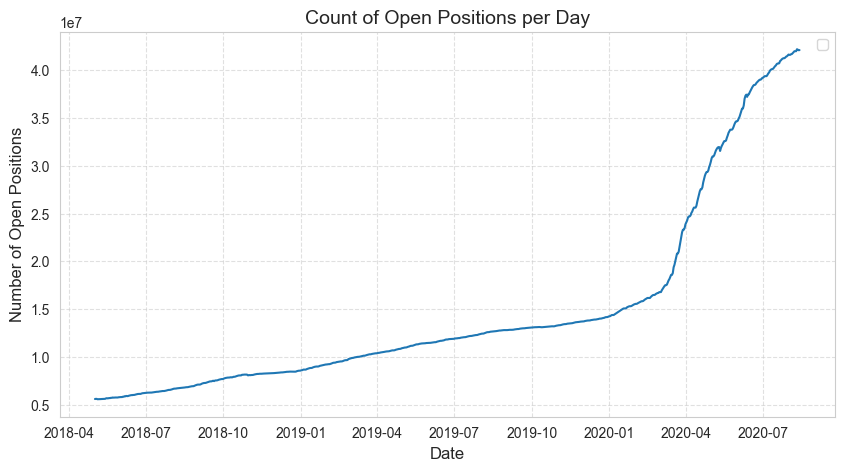
\includegraphics[width=1\linewidth]{../images/old/no_positions_date.png}
    \caption{Daily count of open Robinhood positions, May 2018-August 2020.}
\end{figure}

The figure above shows the daily count of open positions on Robinhood from April 2018 to mid-2020. 
We observe a steady increase in user participation, with a sharp acceleration beginning in early 2020. 
This surge coincides with the onset of the COVID-19 pandemic, likely driven by a combination of heightened market volatility, increased retail interest, and fiscal stimulus payments.
